\section{多边形的定义}
\subsection{正方形顶点的定义} \label{def_square}
前面我们已经看到如何定义一些三角形。下面来看一些四边形和正多边形。

\begin{NewMacroBox}{tkzDefSquare}{\parg{pt1,pt2}}%
给定两个点，可再得到两个点，使这四个点按顺序构成一个正方形；正方形按逆时针方向定义。\\结果分别保存在 \tkzname{tkzFirstPointResult} 和 \tkzname{tkzSecondPointResult} 中。\\
可用 \tkzcname{tkzGetPoints} 为它们重新命名。

\medskip
\begin{tabular}{lll}%
\toprule
参数             & 示例 & 说明                         \\ 
\midrule
\TAline{\parg{pt1,pt2}}{\tkzcname{tkzDefSquare}\parg{A,B}}{正方形按逆时针方向定义。}
\end{tabular}
\end{NewMacroBox}

\subsubsection{用两个点调用 \tkzcname{tkzDefSquare}}
注意交换前两个点会得到不同结果。

\begin{tkzexample}[latex=4cm,small]
\begin{tikzpicture}[scale=.5]
  \tkzDefPoint(0,0){A} \tkzDefPoint(3,0){B}
  \tkzDefSquare(A,B)
  \tkzDrawPolygon[new](A,B,tkzFirstPointResult,%
               tkzSecondPointResult)
  \tkzDefSquare(B,A)
  \tkzDrawPolygon(B,A,tkzFirstPointResult,%
               tkzSecondPointResult) 
\end{tikzpicture} 
\end{tkzexample}

有时我们可能只需要其中一个点，用来绘制等腰直角三角形，这时可使用 \\ \tkzcname{tkzGetFirstPoint} 或 \tkzcname{tkzGetSecondPoint}。

\subsubsection{用 \tkzcname{tkzDefSquare} 得到等腰直角三角形}
\begin{tkzexample}[latex=7cm,small]
\begin{tikzpicture}[scale=1]
  \tkzDefPoint(0,0){A}
  \tkzDefPoint(3,0){B}
  \tkzDefSquare(A,B) \tkzGetFirstPoint{C}
  \tkzDrawSegment(A,B)
  \tkzDrawSegments[new](A,C B,C)
  \tkzMarkRightAngles(A,B,C)
  \tkzDrawPoints(A,B) \tkzDrawPoint[new](C)
  \tkzLabelPoints(A,B)
  \tkzLabelPoints[new,above](C)
\end{tikzpicture}
\end{tkzexample}

\subsubsection{勾股定理与 \tkzcname{tkzDefSquare}}
\begin{tkzexample}[latex=8cm,small]
\begin{tikzpicture}[scale=.5]
\tkzDefPoint(0,0){C}
\tkzDefPoint(4,0){A}
\tkzDefPoint(0,3){B} 
\tkzDefSquare(B,A)\tkzGetPoints{E}{F} 
\tkzDefSquare(A,C)\tkzGetPoints{G}{H} 
\tkzDefSquare(C,B)\tkzGetPoints{I}{J} 
\tkzDrawPolygon(A,B,C) 
\tkzDrawPolygon(A,C,G,H) 
\tkzDrawPolygon(C,B,I,J) 
\tkzDrawPolygon(B,A,E,F) 
\tkzLabelSegment(A,C){$a$} 
\tkzLabelSegment[right](C,B){$b$} 
\tkzLabelSegment[swap](A,B){$c$} 
\end{tikzpicture}
\end{tkzexample}

\subsection{矩形顶点的定义}
。

\begin{NewMacroBox}{tkzDefRectangle}{\parg{pt1,pt2}}%
给定两个点，可再得到两个点，使这四个点按顺序构成一个矩形；矩形按逆时针方向定义。作为参数给出的两个点是一条对角线的两个端点，矩形的各边分别平行于坐标轴。\\
 结果保存在 \tkzname{tkzFirstPointResult} 和 \tkzname{tkzSecondPointResult} 中。\\
可用 \tkzcname{tkzGetPoints} 为它们重新命名。

\medskip
\begin{tabular}{lll}%
\toprule
参数             & 示例 & 说明                         \\ 
\midrule
\TAline{\parg{pt1,pt2}}{\tkzcname{tkzDefRectangle}\parg{A,B}}{矩形按逆时针方向定义。}
\end{tabular}
\end{NewMacroBox}

\subsubsection{矩形定义示例}
\begin{tkzexample}[latex=7 cm,small]
\begin{tikzpicture}
\tkzDefPoints{0/0/A,5/2/C}
\tkzDefRectangle(A,C) \tkzGetPoints{B}{D}
\tkzDrawPolygon[fill=teal!15](A,...,D)
\end{tikzpicture}
\end{tkzexample}

\subsection{平行四边形的定义} 

定义平行四边形的顶点：由给定的三个点补出第四个点。
\begin{NewMacroBox}{tkzDefParallelogram}{\parg{pt1,pt2,pt3}}%
\begin{tabular}{lll}%
\toprule
参数 &  默认值 & 含义  \\ 
\midrule
\TAline{\parg{pt1,pt2,pt3}}{无默认}{需要给出三个点}
\bottomrule
\end{tabular}
\end{NewMacroBox}

由三个点可得到另一个点，使这四个点按顺序构成一个平行四边形。
\\ 结果保存在 \tkzname{tkzPointResult} 中。\\
可用 \tkzcname{tkzGetPoint} 为它重新命名。


\subsubsection{平行四边形定义示例}

\begin{tkzexample}[latex=7 cm,small]
\begin{tikzpicture}[scale=1]
 \tkzDefPoints{0/0/A,3/0/B,4/2/C} 
 \tkzDefParallelogram(A,B,C) 
 % or   \tkzDefPointWith[colinear= at C](B,A) 
 \tkzGetPoint{D}
 \tkzDrawPolygon(A,B,C,D)
 \tkzLabelPoints(A,B) 
 \tkzLabelPoints[above right](C,D)
 \tkzDrawPoints(A,...,D)
\end{tikzpicture}
\end{tkzexample}


\subsection{黄金矩形} 
 \begin{NewMacroBox}{tkzDefGoldenRectangle}{\parg{point,point}}%
本宏确定一个矩形，使其邻边之比为 $\Phi$。\\
 新生成的点保存在 \tkzname{tkzFirstPointResult} 和 \tkzname{tkzSecondPointResult} 中。\\
 可用宏 \tkzcname{tkzGetPoints} 取出它们。

\begin{tabular}{lll}%
\toprule
参数             & 示例 & 说明                         \\
\midrule
\TAline{\parg{pt1,pt2}}{\parg{A,B}}{若新生成 C、D，则 $AB/BC=\Phi$。}
 \end{tabular}
 
 \tkzcname{tkzDefGoldenRectangle} 或 \tkzcname{tkzDefGoldRectangle}
\end{NewMacroBox}


\subsubsection{黄金矩形}
\begin{tkzexample}[latex=6 cm,small]
\begin{tikzpicture}[scale=.6]
 \tkzDefPoint(0,0){A}      \tkzDefPoint(8,0){B}
 \tkzDefGoldRectangle(A,B) \tkzGetPoints{C}{D}
 \tkzDefGoldRectangle(B,C) \tkzGetPoints{E}{F}
 \tkzDefGoldRectangle(C,E) \tkzGetPoints{G}{H}
 \tkzDrawPolygon(A,B,C,D)
 \tkzDrawSegments(E,F G,H)
\end{tikzpicture}
\end{tkzexample}

\subsubsection{黄金矩形的尺规作法}
下面给出不使用上述宏来构造黄金矩形的方法。

\begin{tkzexample}[latex=8cm,small]
\begin{tikzpicture}[scale=.5] 
\tkzDefPoint(0,0){A}
\tkzDefPoint(8,0){B} 
\tkzDefMidPoint(A,B)
\tkzGetPoint{I} 
\tkzDefSquare(A,B)\tkzGetPoints{C}{D} 
\tkzInterLC(A,B)(I,C)\tkzGetPoints{G}{E} 
\tkzDefPointWith[colinear= at C](E,B) 
 \tkzGetPoint{F}
\tkzDefPointBy[projection=onto D--C ](E) 
 \tkzGetPoint{H}
\tkzDrawArc[style=dashed](I,E)(D)
\tkzDrawPolygon(A,B,C,D) 
\tkzDrawPoints(C,D,E,F,H) 
\tkzLabelPoints(A,B,C,D,E,F,H)
\tkzLabelPoints[above](C,D,F,H)  
\tkzDrawSegments[style=dashed,color=gray]%
(E,F C,F B,E F,H H,C E,H) 
\end{tikzpicture}
\end{tkzexample}




\subsection{正多边形} 
 \begin{NewMacroBox}{tkzDefRegPolygon}{\oarg{local options}\parg{pt1,pt2}}%
给定边数后，本宏根据所选选项，从中心或从一条边出发确定一个正多边形。

\begin{tabular}{lll}%
\toprule
参数             & 示例 & 说明                         \\
\midrule
\TAline{\parg{pt1,pt2}}{\parg{O,A}}{配合选项 \code{center}，$O$ 为正多边形的中心。}
\TAline{\parg{pt1,pt2}}{\parg{A,B}}{配合选项 \code{side}，$[AB]$ 为正多边形的一条边。}
 \end{tabular}

\medskip
\begin{tabular}{lll}%
\toprule
选项             & 默认值 & 示例                         \\
\midrule
\TOline{name}{P}{顶点命名为 $P1$、$P2$、……}
\TOline{sides}{5}{边数。}
\TOline{center}{center}{第一个点为中心。}
\TOline{side}{center}{给出的两个点为顶点。}
\TOline{Options TikZ}{...}{}
\end{tabular} 
\end{NewMacroBox}

\subsubsection{选项 \tkzname{center}}
\begin{tkzexample}[latex=7cm, small]   
\begin{tikzpicture}
  \tkzDefPoints{0/0/P0,0/0/Q0,2/0/P1}
  \tkzDefMidPoint(P0,P1) \tkzGetPoint{Q1}
  \tkzDefRegPolygon[center,sides=7](P0,P1)
  \tkzDefMidPoint(P1,P2) \tkzGetPoint{Q1}
  \tkzDefRegPolygon[center,sides=7,name=Q](P0,Q1)
  \tkzFillPolygon[teal!20](Q0,Q1,P2,Q2)
  \tkzDrawPolygon(P1,P...,P7)
  \foreach \j in {1,...,7} {%
  \tkzDrawSegment[black](P0,Q\j)}
\end{tikzpicture}
\end{tkzexample}

\subsubsection{选项 \tkzname{side}}
\begin{tkzexample}[latex=7cm, small]   
\begin{tikzpicture}[scale=1]
    \tkzDefPoints{-4/0/A, -1/0/B}
    \tkzDefRegPolygon[side,sides=5,name=P](A,B)
    \tkzDrawPolygon[thick](P1,P...,P5)
\end{tikzpicture}
\end{tkzexample}
\endinput
